\section{Experiments} \label{sec:experiments}

In this section we will compare the training time of the proposed tree training algorithm with the traditional training algorithm. Note that for each of the experiments below we verified that the decision trees returned by two algorithms are identical. In the first part of the experiments we have tested our proposed algorithm on some real data and compared the running time to the traditional tree training algorithm as it was used in \emph{scikit-learn} before our change was incorporated in. In the second part of the experiment we tested our algorithm on some synthetic data with varying density to show how our algorithm can benefit from sparsity. Note that the density of a dataset is the percentage of its non-zero values. \\\\

\subsection{Density}
The density of a matrix $X$ is the percentage of its nonzero entries and the sparsity is the percentage of its zero entries. As we will see below training of decision trees on datasets that are quite sparse (with density below $0.01$) is significantly faster using our algorithm. Furthermore in the \emph{Synthetic Data} section we compare running time of decision trees with sparse csc matrices and dense arrays as a function of density. Note that in all the experiments below we made sure that both algorithms (induction of decision trees with a sparse csc matrix and the traditional induction of decision trees with dense arrays) lead exactly to the same model structure and have the same generalization performance.\\\\

\subsection{Real Data}

\begin{figure}[h]
\centering
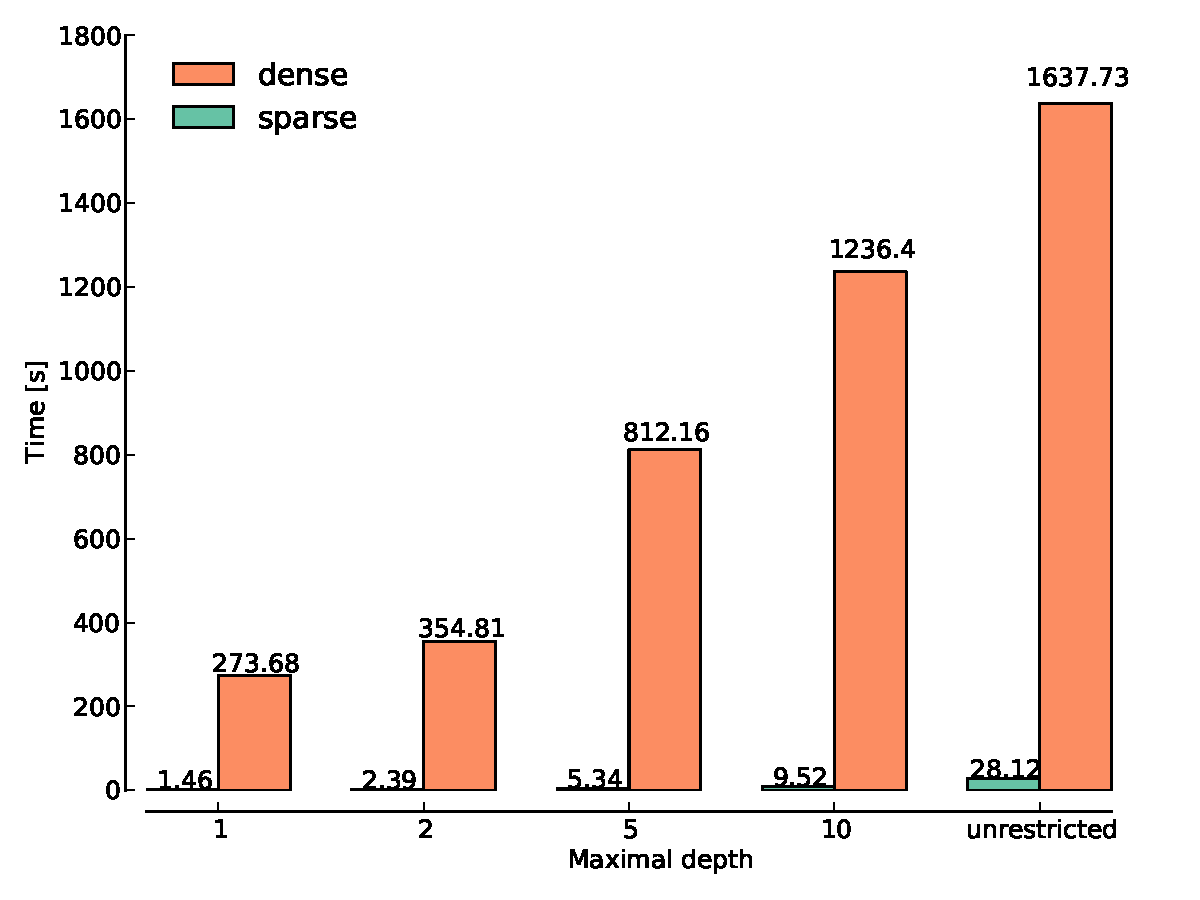
\includegraphics[scale=0.45]{images/20news.pdf}
\caption{Leveraging the input sparsity significantly speed up decisions
         tree induction both with shallow and deep trees on the \emph{20 Newsgroups}
         dataset. Note that the dataset is very sparse (density = 0.001).}
\label{fig:20news}
\end{figure}

\begin{figure}[h]
\centering
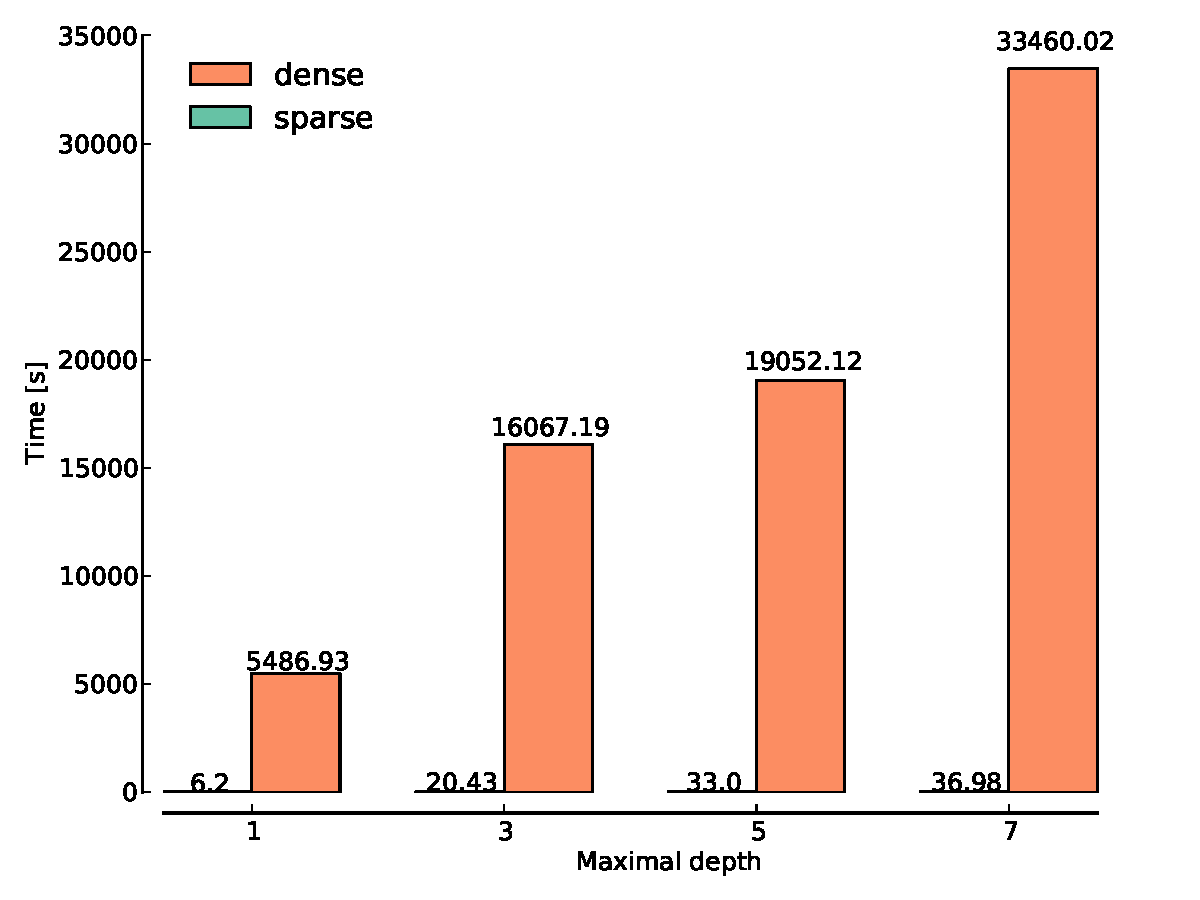
\includegraphics[scale=0.45]{images/cup.pdf}
\caption{Leveraging the input sparsity significantly speed up decisions
         tree induction both with shallow and deep trees on the \emph{cup}
         dataset. Note that the dataset is quite sparse (density = 0.014).}
\label{fig:cup}
\end{figure}


\begin{figure}[h]
\centering
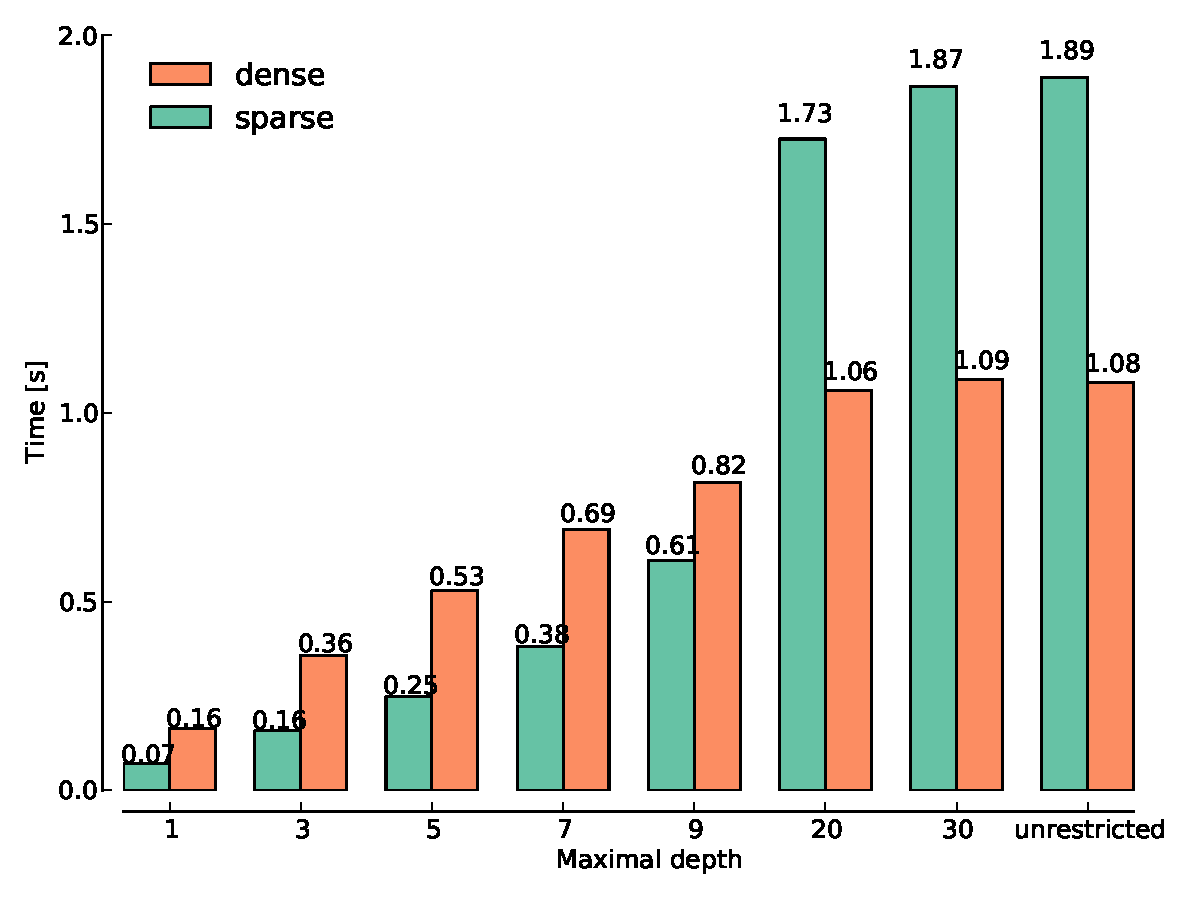
\includegraphics[scale=0.45]{images/adult.pdf}
\caption{Leveraging the input sparsity does not speed up training of deep trees on the \emph{adult}
         dataset. Note that the dataset is quite dense (density = 0.11).}
\label{fig:adult}
\end{figure}


\begin{figure}[h]
\centering
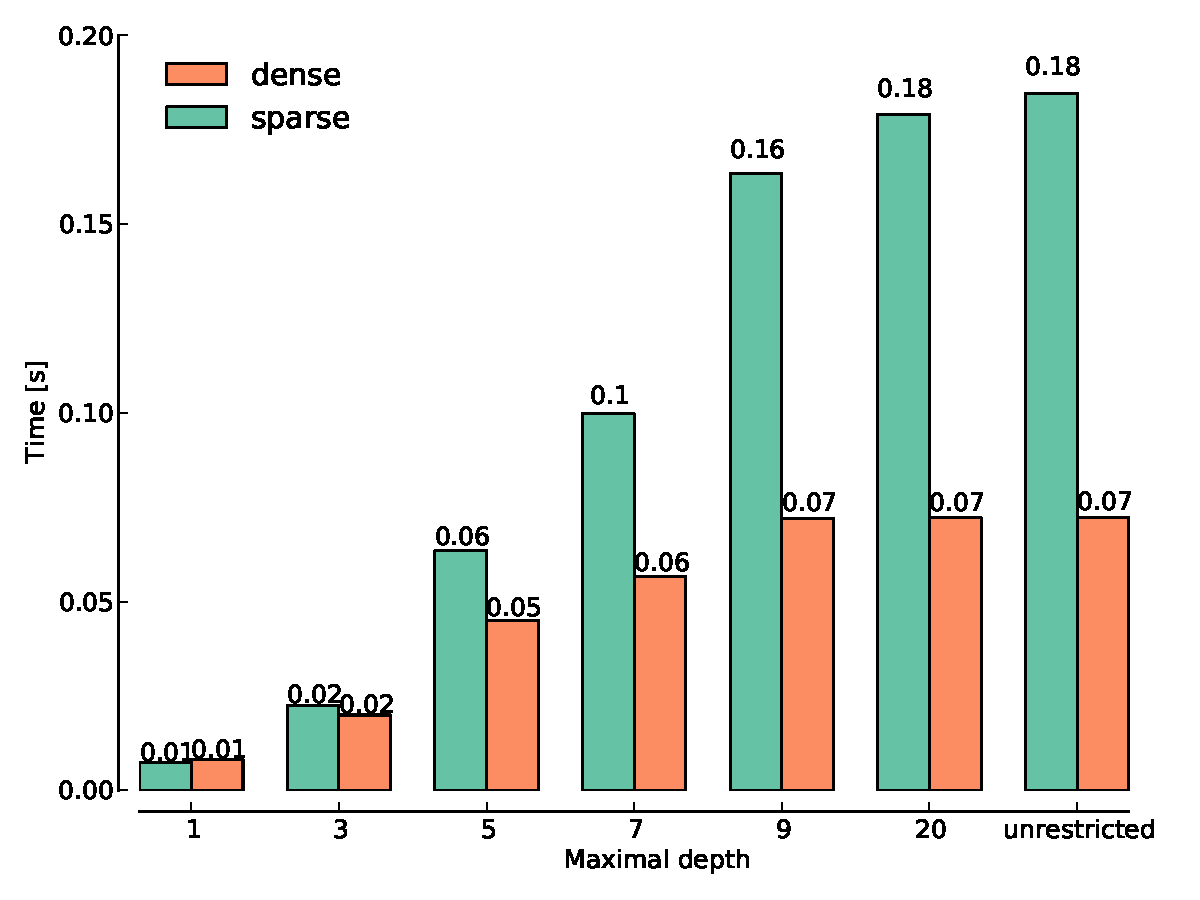
\includegraphics[scale=0.45]{images/tic.pdf}
\caption{Leveraging the input sparsity does not speed up training trees on the \emph{tic}
         dataset. Note that the dataset is very dense (density = 0.44).}
\label{fig:tic}
\end{figure}

In this section we will assess the computational performance of the decision tree algorithm on datasets composed dominantly of categorical or textual features, which makes them very sparse, and on datasets that are more dense. We will compare the learning time between the decision tree learnt
using a sparse csc matrix and a dense array.
The first two experiments are on very sparse datasets, namely on the \emph{20 Newsgroups} dataset \cite{joachims1996probabilistic} and on the \emph{KDD cup 1999} dataset\cite{bay2000archive}. The \emph{20 Newsgroups} dataset
consists of $n=11314$ document on $20$ topics. Each text document was
transformed into sparse tf-idf vectors of size $m=130107$ with a density of
$0.001$. \\
In tree-based ensemble methods, decision trees are either shallow tree as used
in boosting methods or deep tree as random forest ensemble methods. The Figure
\ref{fig:20news} shows that properly taking into account the sparsity of the
input space allows to speed up the learning from 58 times for a fully grown
tree up to 188 times for a decision stump. Furthermore, both algorithm leads
exactly to the same decision tree structure and have the same generalization
performance. The next dataset with low density is the \emph{KDD cup 1999} dataset which consists of $n=96367$ instances. The dataset contains both numerical and categorical data. The feature size of the dataset with categorical features transformed to binary features is $m=20025$ with an average density of
$0.014$. Unlike the previous dataset, the task at hand for this dataset is regression. We will compare the learning time between the decision tree regressor learnt
using a sparse csc matrix and a dense array. As Figure \ref{fig:cup} shows taking into account the sparsity of the
input space allows to speed up the learning by a factor between 800 and 900. Furthermore, both algorithm lead
exactly to the same decision tree regressor structure and have the same generalization
performance.\\

Our dense datasets are the \emph{Adult} dataset\cite{Bache+Lichman:2013} with a density of $0.12$, $n=32561$ instances and  $m=145$ features, and the \emph{TIC} dataset\cite{Bache+Lichman:2013} with a density of $0.44$ and $n=4000$ instances and $m=85$ features. As Figure \ref{fig:adult} shows for shallower trees sparse threes are approximately learnt twice faster than their dense counterparts, but for fully grown threes it is the opposite. Finally as Figure \ref{fig:tic} shows decision threes are learnt faster by dense input data rather than by input data sparsely represented. 


\subsection{Synthetic Data}

\begin{figure}[!h]
\centering
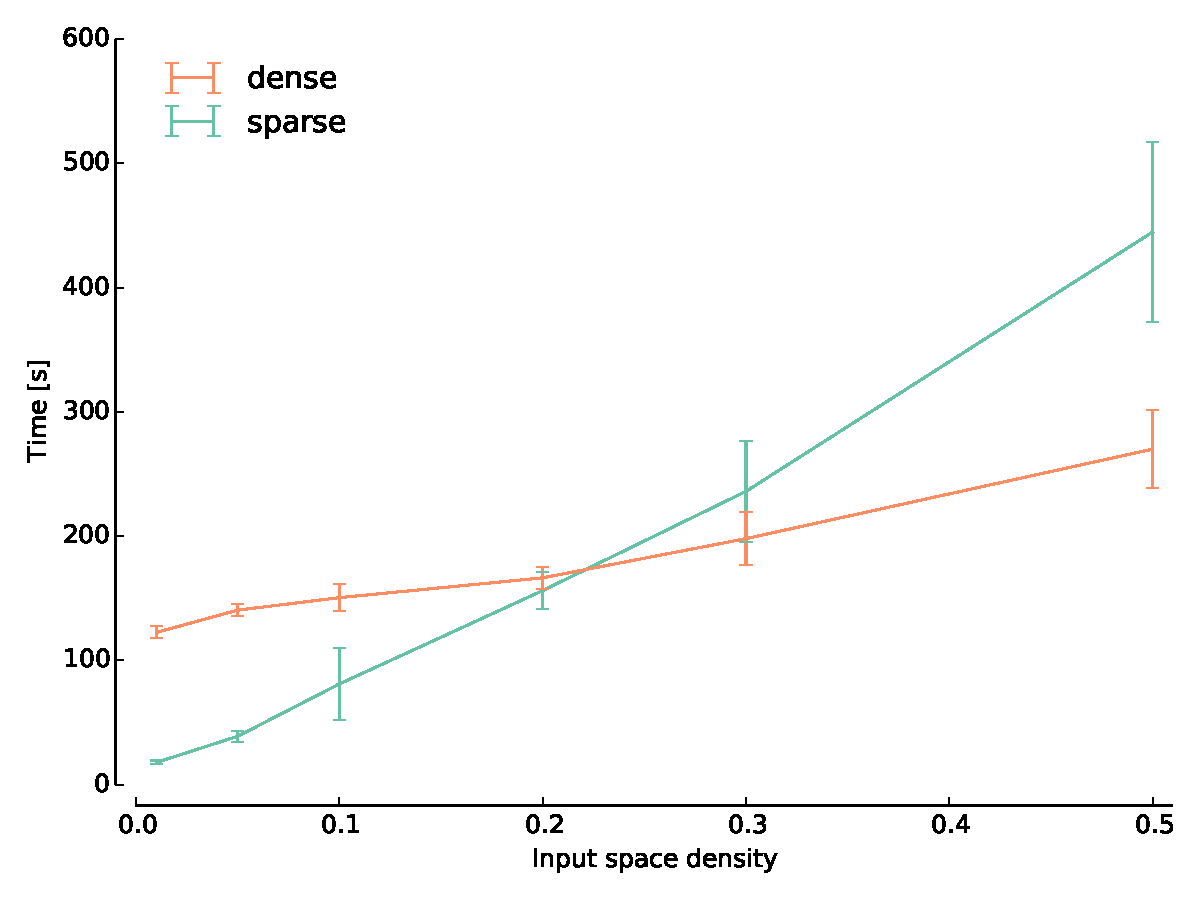
\includegraphics[scale=0.45]{images/density.pdf}
\caption{Significant speed up is achieved by the sparsity-aware decision tree
         algorithm whenever the density is below 0.2 (or sparsity over 0.8).}
\label{fig:density}
\end{figure}

As a another experiment, we generated random binary classification tasks with
$n=100000$ samples and $m=1000$ features. The input matrices are sparse random
matrices whose nonzero elements are drawn uniformly in $[0, 1)$. Their density
are ranging from $0.01$ to $0.5$. Each point is averaged over 20 experiments
and the maximal depth of the decision tree is restricted to 20. As illustrated
on Figure \ref{fig:density}, the sparsity aware decision tree induction
algorithm exploits the sparsity structure to be trained faster than its dense
counterpart. However whenever the input space density is over $0.2$, the
extraction of the nonzero values in the sparse csc matrix becomes expensive.
This suggests that the sparse decision tree induction algorithm is particularly
suited for sparsely representable data such as text documents.



%\begin{figure}[h]
%\centering
%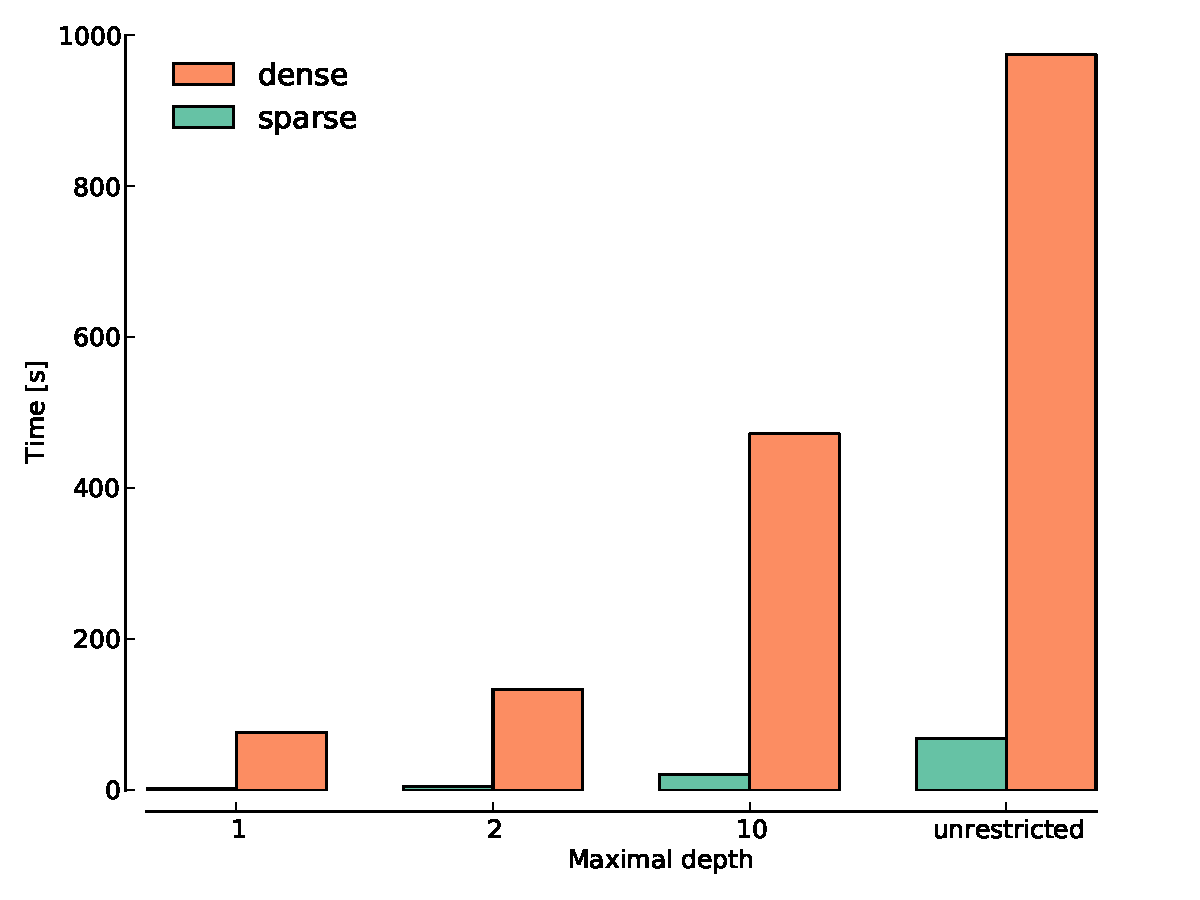
\includegraphics[scale=0.45]{images/depth.pdf}
%\caption{Leveraging the input sparsity significantly speed up decisions
%         tree induction both with shallow and deep trees on the \emph{20 Newsgroups}
%         dataset.}
%\label{fig:depth}
%\end{figure}



